\chapter{Experiments}

\section{BM25}

We used grid search for $k_1 \in [0.2,2.0]$, $b\in[0.1,1.0]$ with the step size of $0.1$, over the training splits.
Only the entries labeled supported and refuted were used since only such entries provide evidence.
We performed fine-tuning over whole training splits for both \CTK{} and FEVER CS datasets.
% For the \CTK{} dataset, we performed the fine-tuning over the whole training split, while for the FEVER CS dataset, we randomly selected 10,000 verifiable claims from the training set.
The resulting parameters were chosen according to the best recall achieved on the training data, calculated by summing up the difference between the best-achieved recall$@k$ and the configuration's recall$@k$.
The monitored levels of the parameter $k$ were 1, 5, 10, 25, 50, 100, and 500. 
The resulting values of the hyperparameters are displayed in Table \ref{tab:bm25_finetune}. 
We note that the difference between the selected values and neighboring values was insignificant (see Table \ref{tab:bm25_sets}). 
%\begin{table}[!htb]
    %\centering
    %\begin{subtable}[t]{.47\textwidth}
        %\centering
        %\begin{tabular}{lrr}
            %datset & $k_1$ & $b$ \\
            %\midrule
            %\CTK{} & 1.0 & 0.5 \\
            %FEVER CS & 1.4 & 0.3
        %\end{tabular}
        %%\caption[BM25 Fine-tuned Parameters]{Fine-tuned parameters for BM25.}
        %%\label{tab:bm25_finetune}
    %\end{subtable}
    %\hfill
    %\begin{subtable}[t]{.47\textwidth}
        %\centering
        %\begin{tabular}{lcc}
            %datset & $k_1$ & $b$ \\
            %\midrule
            %\CTK{} & [0.9, 1.1] & [0.4, 0.5] \\
            %FEVER CS & [1.3, 1.5] & [0.3, 0.4]
        %\end{tabular}
        %%\caption[BM25 Promising Parameter Sets]{Neighbourhoods of parameter values with best results on the training sets.}
        %%\label{tab:bm25_sets}
    %\end{subtable}
    %\caption[BM25 Parameter Selection]{Results of BM25 fine-tuning. \textbf{Left}: The selected fine-tuned parameters. \textbf{Right}: Neighbourhoods of parameter values with the best performance.}
%\end{table}
\begin{table}[!htb]
    \centering
    \begin{minipage}[t]{.47\textwidth}    
        \centering
        \begin{tabular}{lrr}
            datset & $k_1$ & $b$ \\
            \midrule
            \CTK{} & 1.0 & 0.5 \\
            FEVER CS & 1.4 & 0.3
        \end{tabular}
        \caption[BM25 Fine-tuned Parameters]{Fine-tuned parameters for BM25.}
        \label{tab:bm25_finetune}
    \end{minipage}
    \hfill
    \begin{minipage}[t]{.47\textwidth}
        \centering
        \begin{tabular}{lcc}
            datset & $k_1$ & $b$ \\
            \midrule
            \CTK{} & [0.9, 1.1] & [0.4, 0.5] \\
            FEVER CS & [1.3, 1.5] & [0.3, 0.4]
        \end{tabular}
        \caption[BM25 Promising Parameter Sets]{Neighbourhoods of parameter values with the best performance.}
        \label{tab:bm25_sets}
    \end{minipage}
\end{table}

\section{ColBERT and mBERT baselines}

We used the ColBERT and mBERT models pre-trained and fine-tuned by \citet{rypar}.
\citet{rypar} performed document retrieval on a paragraph level, and therefore to better compare the models quality in the context of this thesis, we modify the predicted sequences by substituting paragraphs with the document they originate from.
The created duplicates in the predictions are omitted in a forward pass, starting from the top and deleting each article we have already encountered.
The change in the resulting metric, however, turned out to be marginal.

\section{\nystr{}}

For \nystr, we used the compact containerized implementation published by the authors\footnote{\url{https://github.com/mlpen/Nystromformer/}}.
The training was done using the MLM task on Czech data, namely Czech Wikipedia\footnote{\url{https://dumps.wikimedia.org/}}, a very large Czech corpus ``czes'' \citet{czes}, and the Corpus of contemporary written (printed) Czech ``SYN v4'' \citep{syn}. 
The reason for such a large amount of data is that when using inputs of length 2048 tokens, we obtain a relatively small number of instances, and the fact that large corpora tend to produce better-performing models \citep{xlmr}.

The model was not trained from scratch; instead, we used the pre-trained RobeCzech model as the starting point. RobeCzech's tokenizer was used, and all the weights, except for the attention mechanism, were initialized as a copy of RobeCzech's weights.
However, we had to address an issue regarding RobeCzech's tokenizer, where the size of the word in its vocabulary was greater than the number of possible tokens. 
This initialization proved to increase the speed of training.
The issue occurred as the vocabulary mapped multiple tokens to \texttt{[UNK]}, a token representing unknown values.
Using a simple wrapper, which returned the correct vocabulary size, around the tokenizer resolved the issue.

The training itself was performed for 3000 steps on four Tesla V100-SXM2-32GB graphics cards, batch size 8, embedding dimension 768, landmark count 512, and a decaying learning rate 8e-5. Figure \ref{fig:nystr_training} shows that for \nystr{}, the training does not significantly slow down after increasing the input length.

\begin{figure}[!htb]
    \centering
    \begin{minipage}{.49\textwidth}
        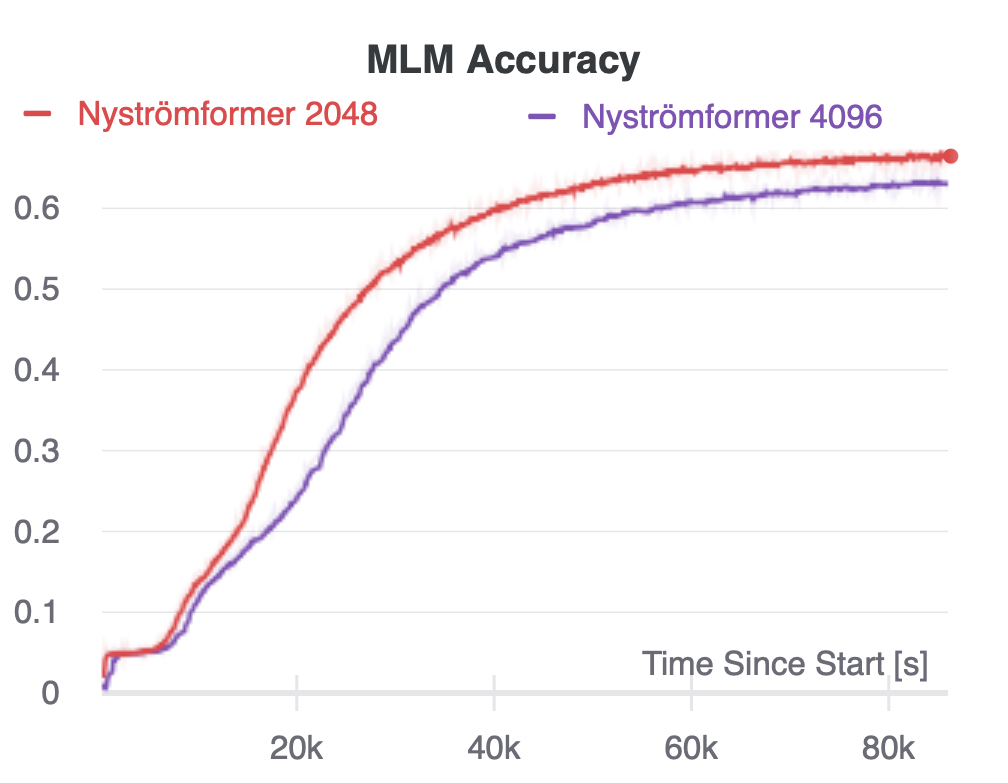
\includegraphics[width=\textwidth]{nystr-train-mlm.png}
    \end{minipage}
    \hfill
    \begin{minipage}{.49\textwidth}
        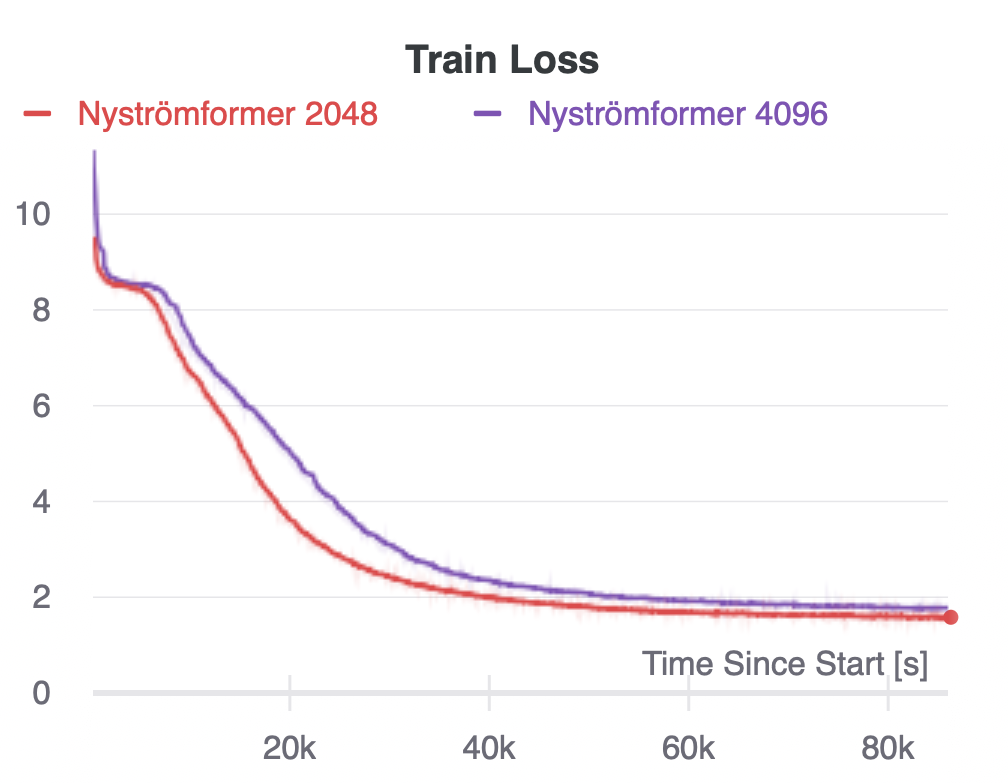
\includegraphics[width=\textwidth]{nystr-train-loss.png}
    \end{minipage}
    \caption[\nystr{} Training]{Comparison of the speed of training for two different input lengths. The experimental setup is the same except for doubled batch size and 1.6 times higher learning rate for the shorter-input model.}
    \label{fig:nystr_training}
\end{figure}

After training, we applied mean-pooling over generated token embeddings to generate the final representations.

\section{BigBird}

We have used the pre-trained BigBird model along with its implementation from the HuggingFace Transformers library \citep{huggingface}. 
We applied multilingual knowledge distillation as described in Section \ref{subsec:distillation} using the SBERT library \citep{sbert}. 
Both the teacher and the student model were initialized as the pre-trained BigBird model.
The training was performed using sentence-parallel Czech-English corpus Czeng 2.0 \citep{czeng2.0}. 
The corpus contains human-translated sentences in both the Czech and the English languages. 
After training for 25 mini-epochs on a single V100 GPU, with a learning rate of 2e-5, and a beth size of 16, the evaluation error stopped decreasing.

The second stage was the training of representation generation, described in Section \ref{subsub:genrep}, again using SBERT.
The model was tasked with generating similar or dissimilar representations of sentences in the Stanford Natural Language Inference (SNLI) Corpus \citep{snli}, depending on the label.
The dataset consists of pairs of sentences labeled \texttt{entailment}, \texttt{contradiction}, and \texttt{neutral}.
The training was performed for 30 epochs.

We theorize that it would be beneficial to train the model on longer inputs than single sentences since BigBird, with its long input capability, cannot train the weights corresponding to the farther parts of the input.
Chaining multiple sentences together from the Czeng 2.0 dataset would not be helpful, as the sentences rarely form a large block of coherent text.
We would thus need a large parallel dataset with whole works translated.
We are, however, not aware of such a Czech-English dataset.

\section{RobeCzech Baseline}

As a simple baseline we decided to apply the above mentioned method of ``entailment training'' on the SNLI dataset to the RobeCzech model.
We performed the exact same training as the second stage of BigBird training.

\section{Results}


% FINETUNED
% FEVER
% model __@1    __@2    __@5    _@10    _@20	@500
% PRE   0.31	0.20	0.10	0.06	0.03	0.0
% REC   0.29	0.38	0.48	0.53	0.56	0.64
% MRR   0.30	0.34	0.37	0.38	0.38	0.3
% CTK
% PRE   0.24	0.16	0.08	0.05	0.03	0.0
% REC   0.24	0.30    0.39	0.46	0.54	0.8
% MRR   0.21	0.24	0.26	0.27	0.27	0.28

% \begin{table}[!htb]
%     \centering
%     \begin{tabular}{lrrrrrr}
%         \toprule
%             model   & P@1   & P@2	& P@5	& P@10	& P@20	& P@500 \\
%         \midrule
%             BM25 	& 31.13	& 20.36	& 10.41	& 5.80	& 3.09	& 0.14 \\ 
%             mBERT 	& 63.88	& 40.59	& 19.09	& 10.21	& 5.31	& 0.23 \\
%             ColBERT	& 67.25	& 38.74	& 17.41	& 9.16	& 4.76	& 0.21 \\
%         \bottomrule
%     \end{tabular}
%     \caption[FEVER CS Precision]{FEVER CS Precision}
% \end{table}
% 
% \begin{table}[!htb]
% \centering
% \begin{tabular}{lrrrrrr}
%     \toprule
%         model &    R@1 &    R@2 &    R@5 &   R@10 &   R@20 &  R@500 \\
%     \midrule
%          BM25 &  29.09 &  37.55 &  47.70 &  52.64 &  55.91 &  63.52 \\
%         mBERT &  59.60 &  75.28 &  87.55 &  92.84 &  95.47 &  98.89 \\
%       ColBERT &  62.59 &  71.81 &  80.41 &  84.02 &  86.95 &  94.21 \\
%     \bottomrule
% \end{tabular}    
% \caption[FEVER CS Recall]{FEVER CS Recall}
% \end{table}
% 
% \begin{table}[!htb]
%     \centering
%     \begin{tabular}{lrrrrrr}
%     \toprule
%        model &    F@1 &    F@2 &    F@5 &   F@10 &   F@20 &   F@500 \\
%     \midrule
%         BM25 &  30.07 &  26.41 &  17.09 &  10.44 &   5.86 &    0.29 \\
%        mBERT &  61.66 &  52.74 &  31.34 &  18.40 &  10.06 &    0.45 \\
%      ColBERT &  64.84 &  50.33 &  28.62 &  16.52 &   9.03 &    0.42 \\
%     \bottomrule
%     \end{tabular}
%     \caption{FEVER CS F1 Score}
%     \label{tab:fevercs_f1score}
% \end{table}
% 
% \begin{table}[!htb]
%     \centering
%     \begin{tabular}{lrrrrrr}
%         \toprule
%            model &  M@1 &  M@2 &  M@5 &  M@10 &  M@20 &  M@500 \\
%         \midrule
%             BM25 &  29.92 &  34.30 &  37.23 &   37.99 &   38.22 &    38.37 \\
%            mBERT &  56.18 &  63.87 &  67.68 &   68.48 &   68.75 &    68.84 \\
%          ColBERT &  63.93 &  68.41 &  70.70 &   71.16 &   71.34 &    71.47 \\
%         \bottomrule
%         \end{tabular}
%     \caption[FEVER CS MRR]{FEVER CS MRR}
% \end{table}
% 
% \begin{table}[!htb]
%     \centering
%     \begin{tabular}{lrrrrrr}
%         \toprule
%            model &    P@1 &    P@2 &    P@5 &  P@10 &  P@20 &  P@500 \\
%         \midrule
%             BM25 &  24.33 &  15.57 &   8.03 &  4.79 &  2.85 &   0.18 \\
%            mBERT &   9.80 &   7.66 &   5.33 &  3.64 &  2.54 &   0.42 \\
%          ColBERT &  24.37 &  19.22 &  11.11 &  6.91 &  4.20 &   0.38 \\
%         \bottomrule
%         \end{tabular}
%     \caption[\CTK{} Precision]{\CTK{} Precision}
% \end{table}
% 
% \begin{table}[!htb]
%     \centering
%     \begin{tabular}{lrrrrrr}
%         \toprule
%            model &    R@1 &    R@2 &    R@5 &   R@10 &   R@20 &  R@500 \\
%         \midrule
%             BM25 &  24.15 &  29.51 &  38.54 &  45.61 &    54.15 &\bf{80.00}\\
%            mBERT &   9.82 &  14.36 &  20.15 &  25.44 &    32.75 &    72.80 \\
%          ColBERT &  24.43 &  34.26 &  43.58 &  48.61 &\bf{55.16}&    79.35 \\
%         \bottomrule
%         \end{tabular}
%     \caption[\CTK{} Recall]{\CTK{} Recall}
% \end{table}
% 
% \begin{table}[!htb]
%     \centering
%     \begin{tabular}{lrrrrrr}
%     \toprule
%        model &    F@1 &    F@2 &    F@5 &   F@10 &   F@20 &   F@500 \\
%     \midrule
%         BM25 &  24.24 &  20.39 &  13.29 &   8.67 &   5.41 &    0.36 \\
%        mBERT &   9.81 &   9.99 &   8.43 &   6.37 &   4.71 &    0.83 \\
%      ColBERT &  24.40 &  24.63 &  17.70 &  12.10 &   7.80 &    0.75 \\
%     \bottomrule
%     \end{tabular}
%     \caption{\CTK{} F1 Score}
%     \label{tab:ctk_f1score}
% \end{table}
% 
% \begin{table}[!htb]
%     \centering
%     \begin{tabular}{lrrrrrr}
%         \toprule
%            model &  M@1 &  M@2 &  M@5 &  M@10 &  M@20 &  M@500 \\
%         \midrule
%             BM25 &  21.22 &  23.63 &  25.82 &   26.70 &   27.23 &    27.60 \\
%            mBERT &  11.02 &  13.35 &  14.97 &   15.60 &   16.12 &    16.62 \\
%          ColBERT &  23.31 &  28.07 &  30.32 &   31.09 &   31.51 &    31.93 \\
%         \bottomrule
%         \end{tabular}
%     \caption[\CTK{} MRR]{\CTK{} MRR}
% \end{table}

\begin{table}[!htb]
    \centering
    \begin{tabular}{lrrrrrr}
        \toprule
           model &    P@1 &    P@2 &    P@5 &   P@10 &  P@20 &  P@500 \\
        \midrule
            BM25 &  31.13 &  20.36 &  10.41 &   5.80 &  3.09 &   0.14 \\
           mBERT &  63.88 &  40.59 &  19.09 &  10.21 &  5.31 &   0.23 \\
         ColBERT &  67.25 &  38.74 &  17.41 &   9.16 &  4.76 &   0.21 \\
        \midrule
           {}    &    R@1 &    R@2 &    R@5 &   R@10 &   R@20 &  R@500 \\
        \midrule
            BM25 &  29.09 &  37.55 &  47.70 &  52.64 &  55.91 &  63.52 \\
           mBERT &  59.60 &  75.28 &  87.55 &  92.84 &  95.47 &  98.89 \\
         ColBERT &  62.59 &  71.81 &  80.41 &  84.02 &  86.95 &  94.21 \\
        \midrule
           {}    &    F@1 &    F@2 &    F@5 &   F@10 &   F@20 &   F@500 \\
        \midrule
            BM25 &  30.07 &  26.41 &  17.09 &  10.44 &   5.86 &    0.29 \\
           mBERT &  61.66 &  52.74 &  31.34 &  18.40 &  10.06 &    0.45 \\
         ColBERT &  64.84 &  50.33 &  28.62 &  16.52 &   9.03 &    0.42 \\
        \midrule
           {}    &  M@1 &  M@2 &  M@5 &  M@10 &  M@20 &  M@500 \\
        \midrule
            BM25 &  29.92 &  34.30 &  37.23 &   37.99 &   38.22 &    38.37 \\
           mBERT &  56.18 &  63.87 &  67.68 &   68.48 &   68.75 &    68.84 \\
         ColBERT &  63.93 &  68.41 &  70.70 &   71.16 &   71.34 &    71.47 \\
        \bottomrule
        \end{tabular}
    \caption[FEVER CS Metrics]{FEVER CS Metrics}
\end{table}


\begin{table}[!htb]
    \centering
    \begin{tabular}{lrrrrrr}
        \toprule
           model &    P@1 &    P@2 &   P@5 &  P@10 &  P@20 &  P@500 \\
        \midrule
            BM25 &  24.33 &  15.57 &  8.03 &  4.79 &  2.85 &   0.18 \\
           mBERT &   9.80 &   7.41 &  4.07 &  2.56 &  1.63 &   0.18 \\
         ColBERT &  24.37 &  17.09 &  8.69 &  4.87 &  2.76 &   0.19 \\
        \midrule
              {} &    R@1 &    R@2 &    R@5 &   R@10 &   R@20 &  R@500 \\
        \midrule
            BM25 &  24.15 &  29.51 &  38.54 &  45.61 &  54.15 &  80.00 \\
           mBERT &   9.82 &  14.86 &  20.40 &  25.69 &  32.75 &  72.80 \\
         ColBERT &  24.43 &  34.26 &  43.58 &  48.87 &  55.42 &  79.35 \\
        \midrule
              {} &    F@1 &    F@2 &    F@5 &   F@10 &   F@20 &   F@500 \\
        \midrule
            BM25 &  24.24 &  20.39 &  13.29 &   8.67 &   5.41 &    0.36 \\
           mBERT &   9.81 &   9.89 &   6.79 &   4.66 &   3.11 &    0.36 \\
         ColBERT &  24.40 &  22.80 &  14.50 &   8.86 &   5.27 &    0.38 \\
        \midrule
              {} &  M@1 &  M@2 &  M@5 &  M@10 &  M@20 &  M@500 \\
        \midrule
            BM25 &  21.22 &  23.63 &  25.82 &   26.70 &   27.23 &    27.60 \\
           mBERT &  11.02 &  13.67 &  15.18 &   15.78 &   16.28 &    16.82 \\
         ColBERT &  23.31 &  28.07 &  30.35 &   31.17 &   31.61 &    32.04 \\
        \bottomrule
        \end{tabular}
    \caption[\CTK{} Metrics]{\CTK{} Metrics}
\end{table}

\subsection{\CTK}
\subsection{FEVER CS}

\section{Discussion}

Due to non-compatible codebases of different implementations, resource-intesivity of the task, which also 